%! Author = ASUS
%! Date = 3/27/2023

% Preamble
\documentclass[11pt]{article}

% Packages
\usepackage{amsmath}
\usepackage{wasysym}
\usepackage{graphicx}
\usepackage{listings}
\usepackage{xcolor}
\lstset{basicstyle=\ttfamily,
  showstringspaces=false,
  commentstyle=\color{red},
  keywordstyle=\color{blue}
}

\graphicspath{{./images}}

% Document
\begin{document}
    \section{COLMAP}
    \paragraph{COLMAP} is an open source software, implemented by ~\cite{schoenberger2016sfm} and ~\cite{schoenberger2016mvs},
    that provides 3D reconstruction based on 2D images. The software comes with graphical user interface and
    command-line options that let it to be integrated easily with any other projects. It, also, has a great software
    architecture that makes it a powerful and flexible tool with a wide range of options for customization. COLMAP has
    shown a superb performance in compare to other SfM softwares, and it is being used widely in industry for
    core applications such as 3D modeling and robotics.

    \paragraph{Spare and Dense Reconstructions} are both implemented in COLMAP. Sparse reconstruction results in
    the 3D point cloud of only the detected features, while dense reconstruction refers to the point cloud of all
    pixels in the input images. Dense reconstrution is achievable after obtaining sparse reconstruction with camera
    poses. By default, It run PatchMatch algorithm \cite{journals/tog/BarnesSFG09}, and it is a high time-consuming task.
    Through our project, sparse reconstruction is only considered.

    \paragraph{Customization} is the most important feature in this project. Each step of SfM pipline can be executed
    separately. Hence, any other algorithm can be repalced by its defaults. And, any extra steps, like refinements,
    can be added to the pipeline. Moreover, every single default step has a range of options to change, such as
    the maximum number of features and matches, thresholds, different camera settings with fixed camera parameters, etc.
    Here is sample bash code that shows an overview of our customization applied to the feature detection step:

    \begin{lstlisting}[language=bash,caption={colmapsparse.sh},label={lst:lstlisting2}]
        #!/bin/bash

        colmap feature_extractor \
           --database_path $DATASET_PATH/database.db \
           --image_path $DATASET_PATH/images \
           --SiftExtraction.max_image_size 10000 \
           --SiftExtraction.max_num_features 20000 \
           --SiftExtraction.estimate_affine_shape 1 \
           --ImageReader.single_camera 1 \
           --ImageReader.camera_model FULL_OPENCV \
           --ImageReader.camera_params $CALIB_PARAMS_YAML
    \end{lstlisting}

    \paragraph{In our experiment}, COLMAP is used for 3D reconstruction with different settings. Pixel-Perfect
    refinement codes are placed between COLMAP pipeline after initial keypoints detection. Also, we will see that
    by manipulating COLMAP options, it can be used in vSLAM too.

    \newpage
    \section{Data aquisition}

    \paragraph{GoPro cameras} are small, portable, and captures high quality videos in high frame rates. They also, provide
    a programming api that makes it super easy to develop applications based the cameras' output. Hence, they
    are popular in computer vision and robotics researches. In our experiment, the GoPro 9 camera was fixed on
    a bike, and several videos were taken from the city of Padua, while riding through the streets.

    \paragraph{Our dataset} is created from the two videos captured by the following camera settings:

    \begin{enumerate}
        \item
        \begin{itemize}
            \item 10 minutes, 1080p, 60 frames/sec, Undistorted
            \item SfM input images are every 10 frames from the video, means 6 images per second
        \end{itemize}
        \item
        \begin{itemize}
            \item 25 minutes, 2.7k, 60f, wide and distorted
            \item SfM input images are every 15 frames, 2704×1538 dimensions
        \end{itemize}
    \end{enumerate}

    \paragraph{Extra data:} GoPro cameras come with additional information for the captured videos, such as GPS, IMU.
    https://github.com/gopro/gpmf-parser is the application used to extract these data from video files. Sample GPS
    data of the first 5 seconds:

    \begin{lstlisting}[language=bash,caption={gpmf-parser output},label={lst:lstlisting}]
        VIDEO FRAMERATE:
        59.940 with 31860 frames
        PAYLOAD TIME:
          0.000 to 1.001 seconds
        SCALED DATA:
          GPS5 45.406deg, 11.877deg, 19.839m, 2.418m/s, 2.450m/s,
          GPS5 45.406deg, 11.877deg, 19.831m, 2.432m/s, 2.420m/s,
          GPS5 45.406deg, 11.877deg, 19.816m, 2.489m/s, 2.430m/s,
          GPS5 45.406deg, 11.877deg, 19.811m, 2.501m/s, 2.490m/s,
          GPS5 45.406deg, 11.877deg, 19.807m, 2.501m/s, 2.500m/s,
          GPS5 45.406deg, 11.877deg, 19.821m, 2.495m/s, 2.500m/s,
          GPS5 45.406deg, 11.877deg, 19.828m, 2.503m/s, 2.500m/s,
          GPS5 45.406deg, 11.877deg, 19.830m, 2.505m/s, 2.500m/s,
          GPS5 45.406deg, 11.877deg, 19.825m, 2.520m/s, 2.510m/s,
          GPS5 45.406deg, 11.877deg, 19.819m, 2.493m/s, 2.520m/s,
          GPS5 45.406deg, 11.877deg, 19.822m, 2.472m/s, 2.490m/s,
          GPS5 45.406deg, 11.877deg, 19.820m, 2.471m/s, 2.470m/s,
          GPS5 45.406deg, 11.877deg, 19.822m, 2.494m/s, 2.470m/s,
          GPS5 45.406deg, 11.877deg, 19.790m, 2.448m/s, 2.490m/s,
          GPS5 45.406deg, 11.877deg, 19.775m, 2.444m/s, 2.450m/s,
          GPS5 45.406deg, 11.877deg, 19.775m, 2.434m/s, 2.440m/s,
          GPS5 45.406deg, 11.877deg, 19.759m, 2.404m/s, 2.430m/s,
          GPS5 45.406deg, 11.877deg, 19.763m, 2.412m/s, 2.400m/s,
        PAYLOAD TIME:
          1.001 to 2.002 seconds
        SCALED DATA:
          GPS5 45.406deg, 11.877deg, 19.763m, 2.411m/s, 2.410m/s,
          GPS5 45.406deg, 11.877deg, 19.751m, 2.412m/s, 2.410m/s,
          GPS5 45.406deg, 11.877deg, 19.767m, 2.443m/s, 2.410m/s,
          GPS5 45.406deg, 11.877deg, 19.749m, 2.455m/s, 2.440m/s,
          GPS5 45.406deg, 11.877deg, 19.757m, 2.455m/s, 2.460m/s,
          GPS5 45.406deg, 11.877deg, 19.780m, 2.436m/s, 2.460m/s,
          GPS5 45.406deg, 11.877deg, 19.796m, 2.448m/s, 2.440m/s,
          GPS5 45.406deg, 11.877deg, 19.770m, 2.426m/s, 2.450m/s,
          GPS5 45.406deg, 11.877deg, 19.788m, 2.441m/s, 2.430m/s,
          GPS5 45.406deg, 11.877deg, 19.794m, 2.462m/s, 2.440m/s,
          GPS5 45.406deg, 11.877deg, 19.815m, 2.480m/s, 2.460m/s,
          GPS5 45.406deg, 11.877deg, 19.837m, 2.504m/s, 2.480m/s,
          GPS5 45.406deg, 11.877deg, 19.859m, 2.523m/s, 2.500m/s,
          GPS5 45.406deg, 11.877deg, 19.882m, 2.473m/s, 2.520m/s,
          GPS5 45.406deg, 11.877deg, 19.898m, 2.482m/s, 2.470m/s,
          GPS5 45.406deg, 11.877deg, 19.899m, 2.484m/s, 2.480m/s,
          GPS5 45.406deg, 11.877deg, 19.905m, 2.496m/s, 2.480m/s,
          GPS5 45.406deg, 11.877deg, 19.913m, 2.490m/s, 2.500m/s,
          GPS5 45.406deg, 11.877deg, 19.915m, 2.517m/s, 2.490m/s,
        PAYLOAD TIME:
          2.002 to 3.003 seconds
    \end{lstlisting}

    We will see initial pose for cameras can boost SfM pipeline enormously. However, GPS data from GoPro cameras
    are not usable in this process.
    GPS sampling rate is 18 per second. It means there are 18 position data in one second. However, after reviewing
    all GPS data for a long video, we realized that the coordinates are updated every 2 or 3 seconds which is not ideal.
    In SFM, the algorithm finds the coordinates of the camera for each frame. If we want to use GPS data as an initial
    value in SFM, 40 to 60 frames might have the same initial coordinates which doesn't help the algorithm.
    Moreover, GPS data from GPMF metadata has an accuracy of three-tenth of a decimal. We checked this error in
    Google Maps, and the error could be 10 meters. While, SFM has an error of less than a centimeter.

    \paragraph{Reconstruction}: The extracted frames are then grouped into batches and fed into COLMAP SfM pipeline.

    The first dataset is from the undistorted video. For the ease of recalling, we will call this dataset
    "The First dataset". The first dataset is made from 120 frames with resolution of 1920*1088, and size of ~3MB
    for each image. The figure \ref{fig:1ply} is the sparse reconstruction obtained by COLMAP:

    \begin{figure}
    \caption{The First Dataset: Sparse and Dense Point Cloud}
    \centering
    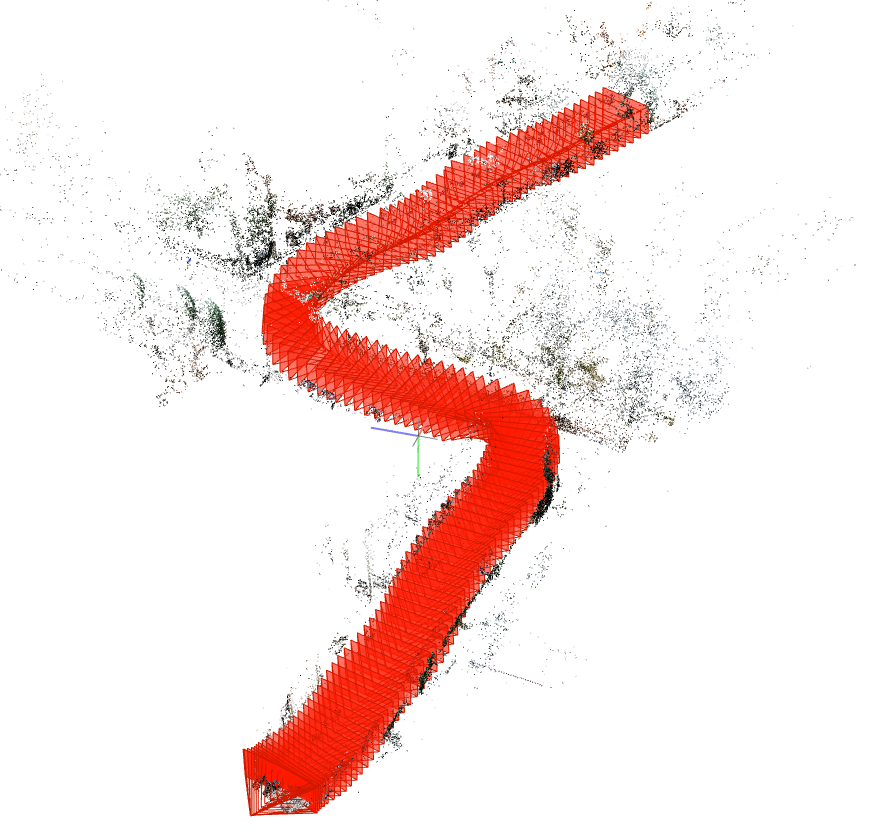
\includegraphics[width=\textwidth,height=\textheight,keepaspectratio]{images/1.ply.sparse.png}
    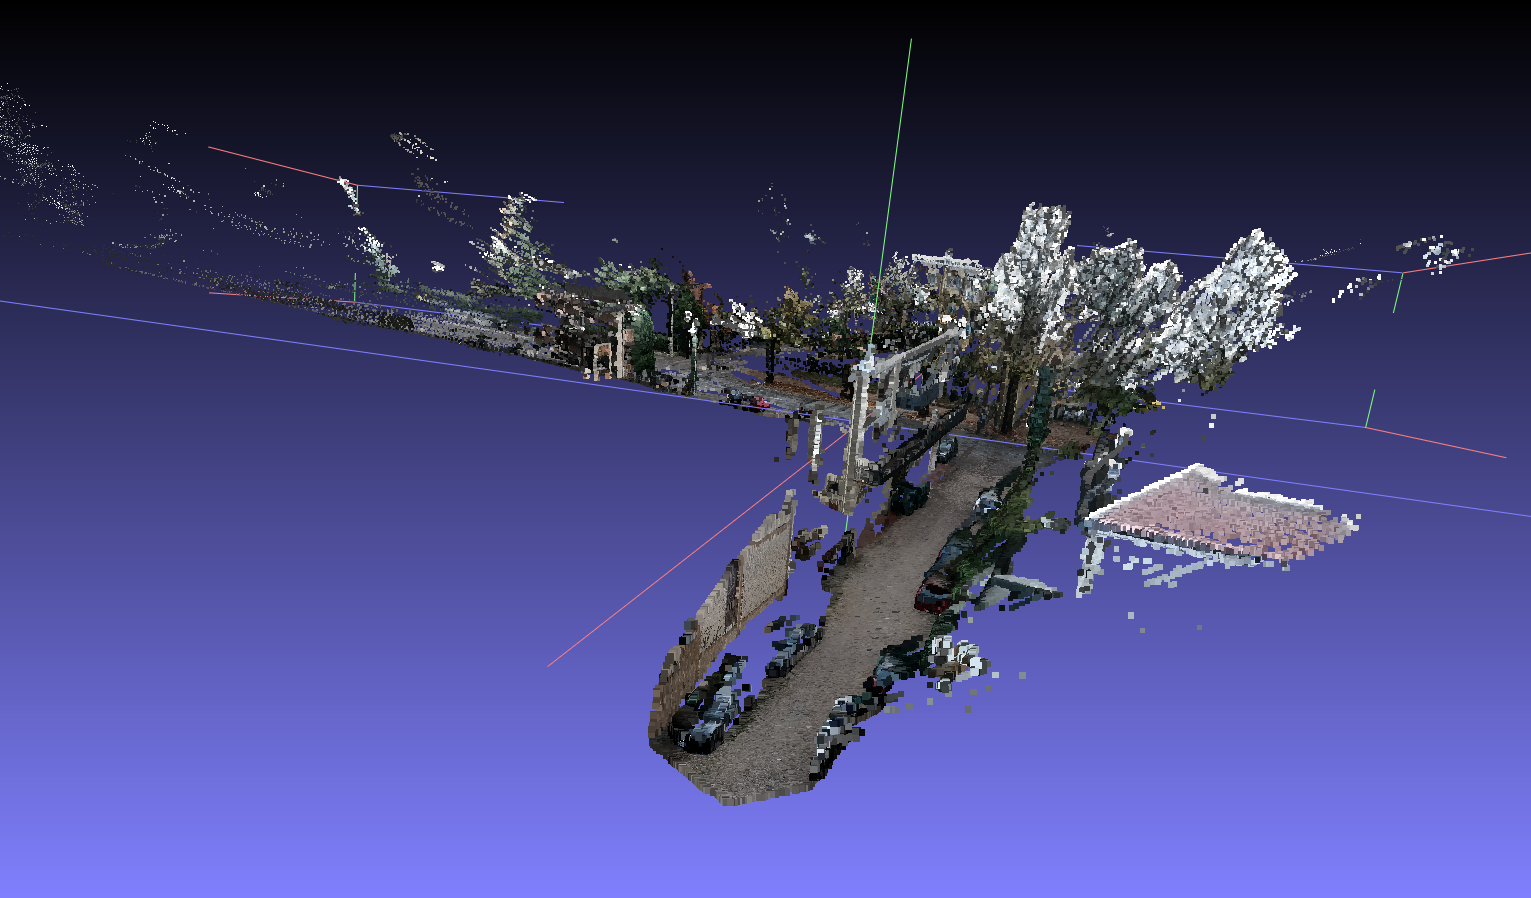
\includegraphics[width=\textwidth,height=\textheight,keepaspectratio]{images/1.ply.dense.1.png}
    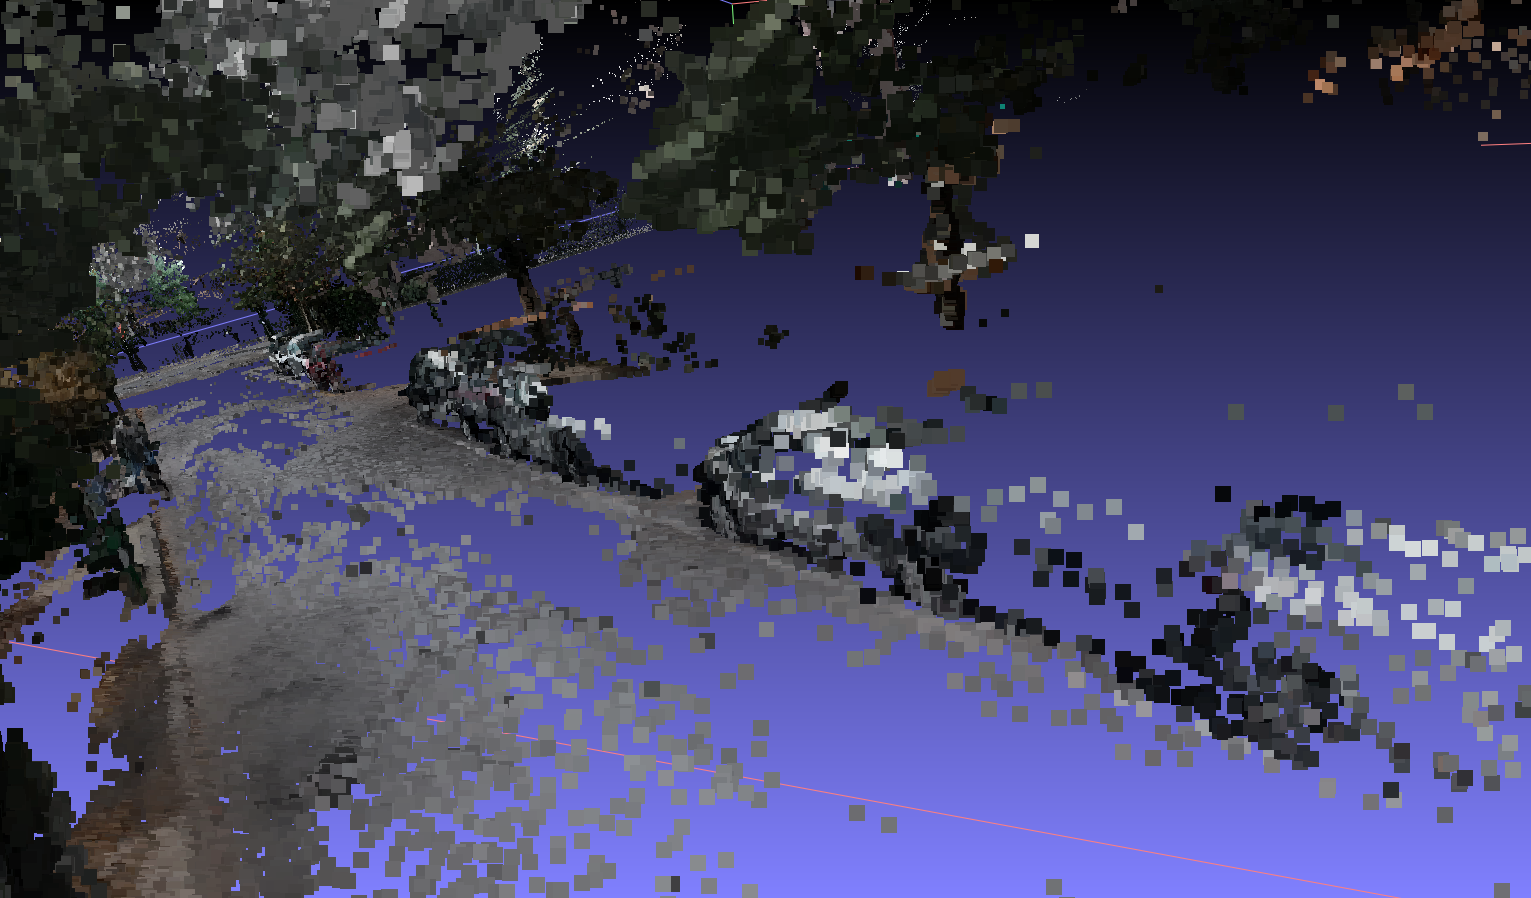
\includegraphics[width=\textwidth,height=\textheight,keepaspectratio]{images/1.ply.dense.2.png}
    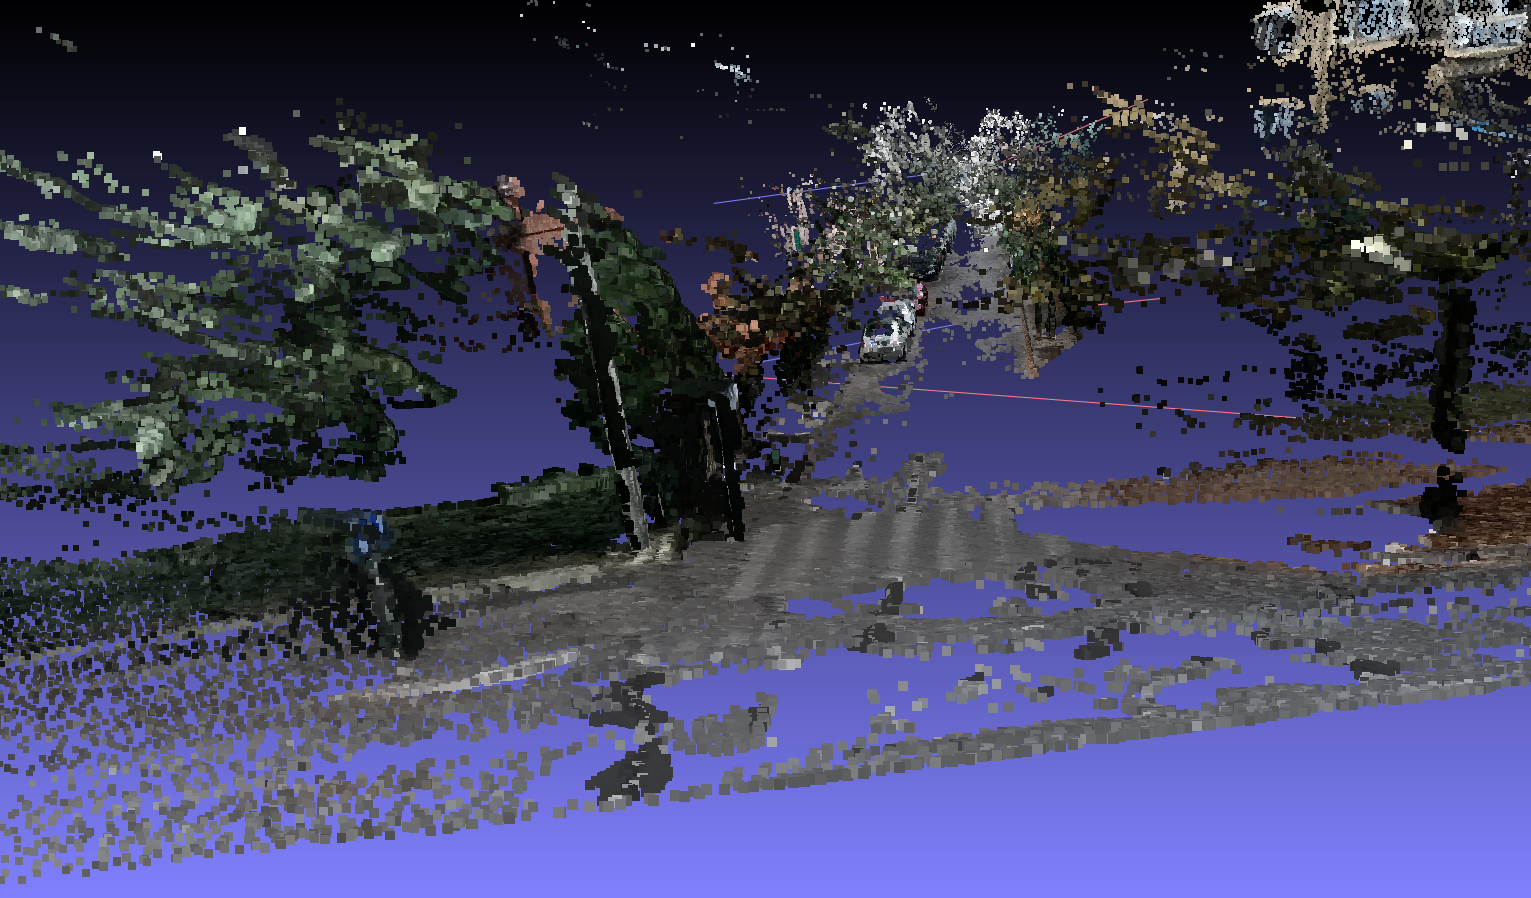
\includegraphics[width=\textwidth,height=\textheight,keepaspectratio]{images/1.ply.dense.3.png}
    \label{fig:1ply}
    \end{figure}

    The Second Dataset is from 2.7k video, and contains 175 distorted images. The final point cloud includes
    100k points. The reconstrution is shown in the figure \ref{fig:2ply}

    \begin{figure}
    \caption{The Second Dataset: Sparse and Dense Point Cloud}
    \centering
    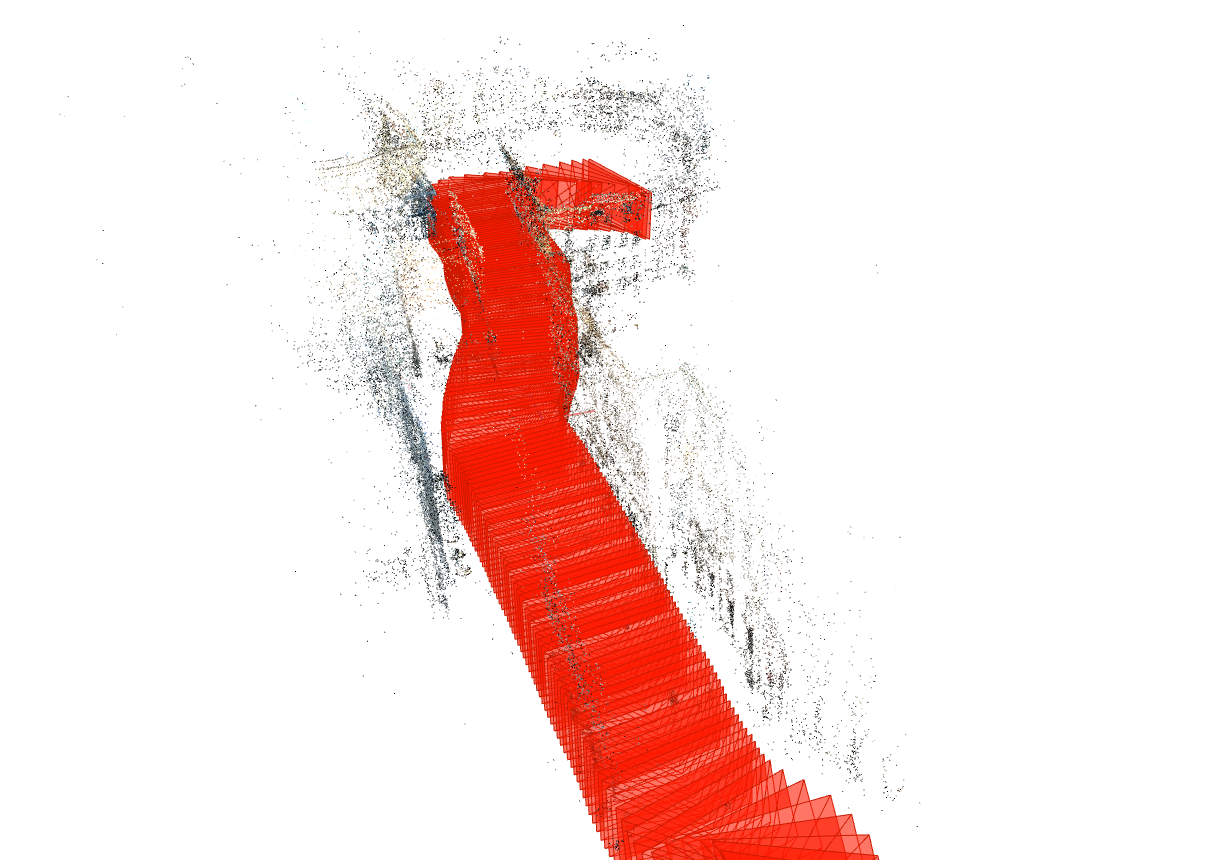
\includegraphics[width=\textwidth,height=\textheight,keepaspectratio]{images/2.ply.sparse.png}
    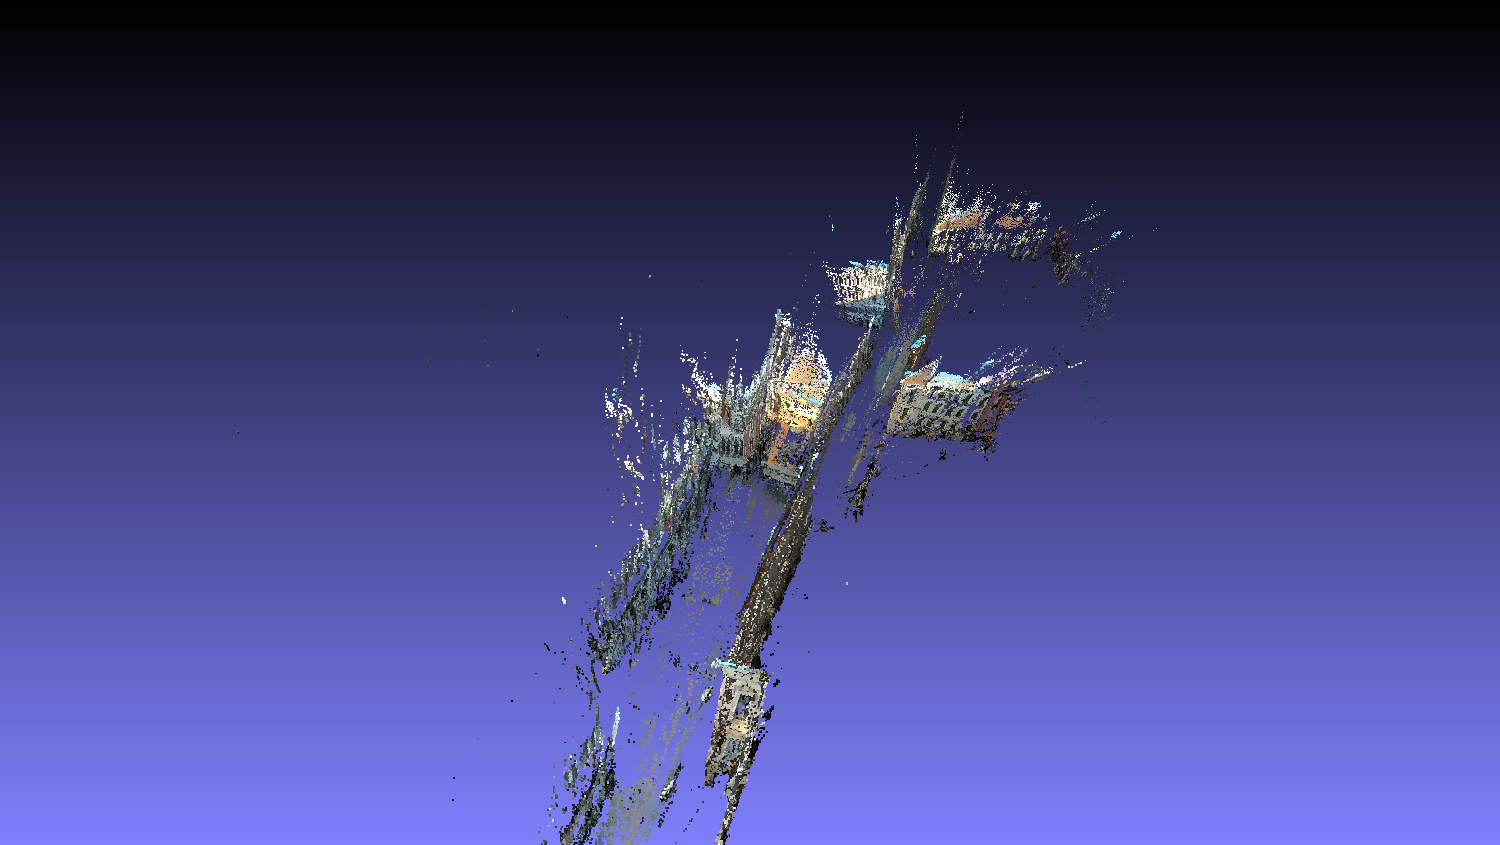
\includegraphics[width=\textwidth,height=\textheight,keepaspectratio]{images/2.ply.dense.1.png}
    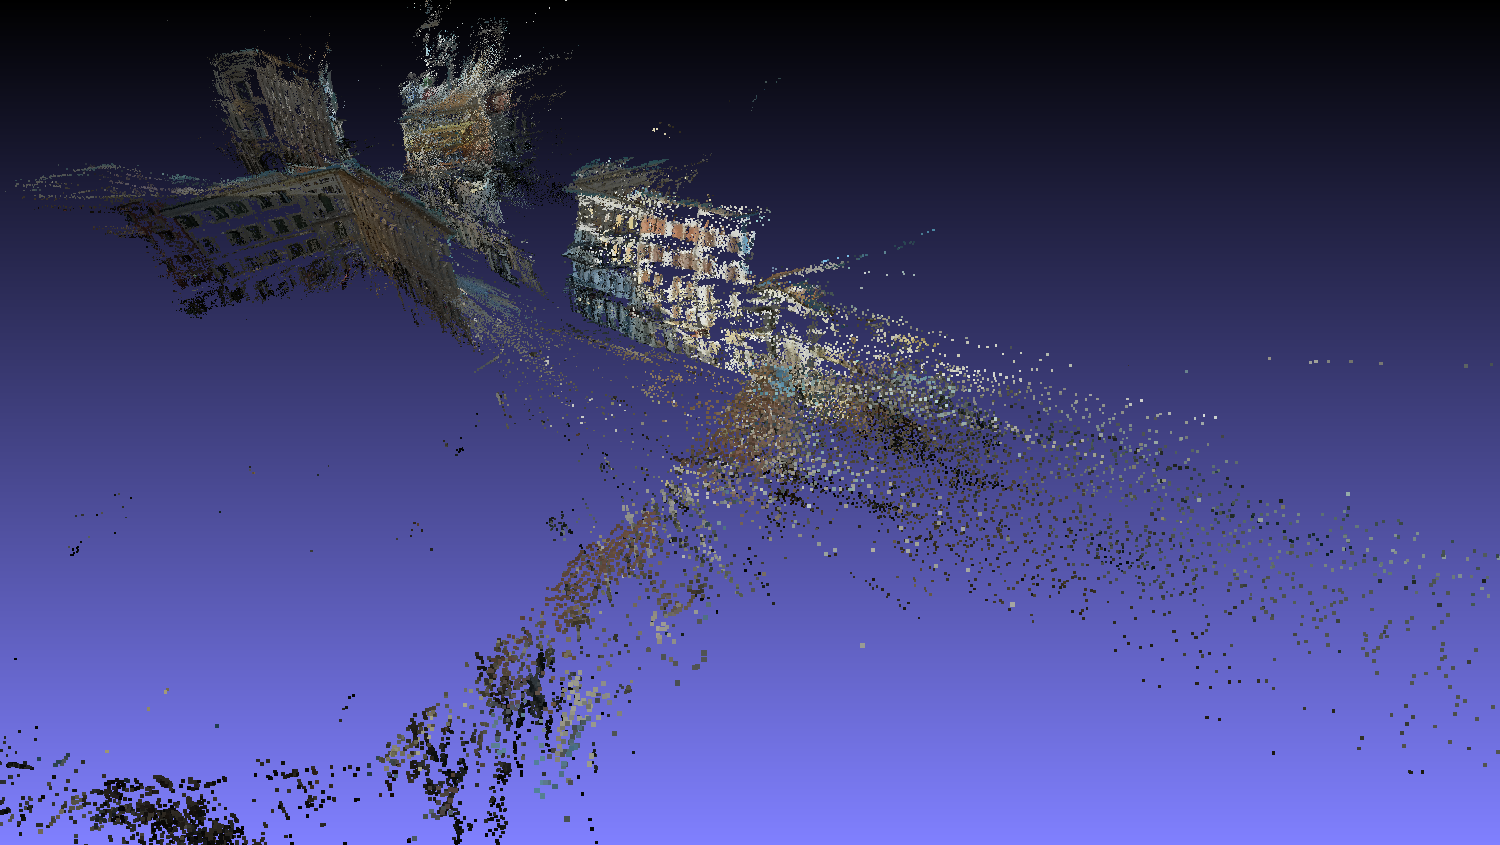
\includegraphics[width=\textwidth,height=\textheight,keepaspectratio]{images/2.ply.dense.2.png}
    \label{fig:2ply}
    \end{figure}

    \section{Refinement}


    \section{Compare the results with City point cloud}
    
    \section{Calibration and its imapct}

    \section{Real-Time Structure from Motion}


\end{document}